 


%\subsubsection*{Objectives}
%\begin{itemize}
%	\item Calculate length of a vector
%	\item Calculate dot products
%	\item Use dot product to determine  
%\end{itemize}



\subsubsection*{Learning outcomes}
Be able to:
\begin{itemize}
	 \item Systematically solve a system of linear equations
	 \item Define: row operations, pivots, over/under-determined systems, row echelon, and reduced row echelon form
	 \item Solve applied problem using elimination
	
\end{itemize}





\rule[0.01in]{\textwidth}{0.0025in}
% ----------------------------------------- % 



% DEFINITION: 
 \begin{tcolorbox}[colback=yellow!10!,colframe=gray!15!]
 \begin{definition}[System of Equations]
A \textbf{linear system} of $m$ equations in $n$ unknowns is then a system of the form
\[ 
\begin{cases} 
a_{11} x_1 + a_{12} x_2 + a_{13} x_3 + \dots + a_{1n} x_n = y_1\\
 a_{21} x_1 + a_{22} x_2 + a_{23} x_3 + \dots + a_{2n} x_n = y_2\\
a_{31} x_1 + a_{32} x_2 + a_{33} x_3 + \dots + a_{3n} x_n = y_3\\

\vdots \\

a_{m1} x_1 + a_{m2} x_2 + a_{m3} x_3 + \dots + a_{mn} x_n = y_m
\end{cases}
\]
 \end{definition}	 
 \end{tcolorbox} 
 
 \begin{tcolorbox}[colback=yellow!10!,colframe=gray!15!]

\begin{definition} (\textbf{Equivalent Systems}) -  Two systems of equations involving the same variables are said to be equivalent if they have the same solution set.  \end{definition}
 \end{tcolorbox} 


\rule[0.01in]{\textwidth}{0.0025in}
% ---------------------------------------------------- % 




\section{Elementary Row Operations} 

There are three elementary row operations that produce  an equivalent system of equations.  


\begin{enumerate}
	\item Interchange two rows
	\item Multiple a row by a nonzero constant
	\item Replace a row by its sum with a multiple of another row
\end{enumerate}

\rule[0.01in]{\textwidth}{0.0025in}
% ---------------------------------------------------- % 


\textbf{Pivot element}: nonzero coefficient of a variable in an equation % (note the singularity of variable and equation)

\textbf{Pivot row}:  Row used to eliminate the elements in other rows % (if the row containing the nonzero pivot element)


%
%%
%%%						  
%%%% SECTION:  Matrices
%%%
%%
%




\begin{example} Solve the system of equations (1 solution):
\[
\begin{array}{rcl} x_1 - 2x_2 & = & 1 \\ 3x_1 +2 x_2 & = &11 \end{array} 
\]

\textbf{Solution}: Use elimination.  (1) Replace the second row by multiplying the first row by $-3$ and adding it to the second.  At this step the system is in \textit{triangular} form and \textbf{back substition} can be used to solve for the unknowns.  

The figures show the original system of equations and the system after performing elementary row operation.  

\[  \begin{array}{rcl} x_1 - 2x_2 & = & 1 \\ 3x_1 +2 x_2 & = &11 \end{array}    \xrightarrow[]{R_2 = -3R_1 + R_2}   \begin{array}{rcl} x_1 - 2x_2 & = & 1 \\  8 x_2 & = & 8 \end{array}   \] 
\end{example}

\begin{figure}[h!]
\centering
\begin{subfigure}{.5\textwidth}
  \centering

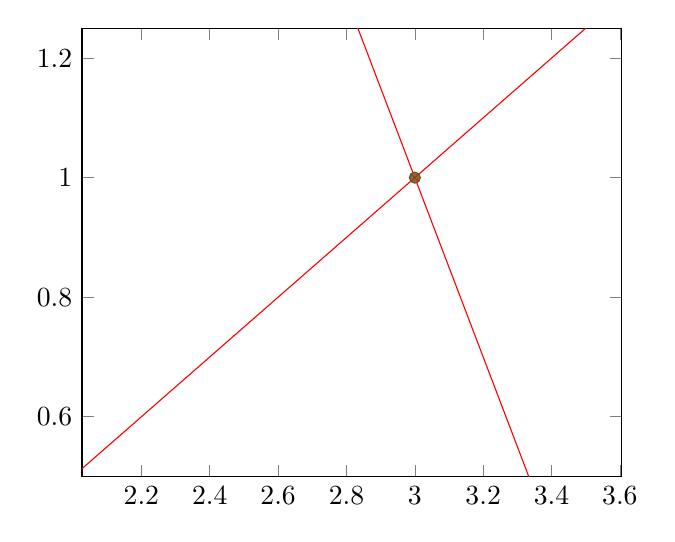
\begin{tikzpicture} \begin{axis}[ymin=0.5,
	ymax=1.25,
]
    % density of Normal distribution:
    \addplot [
        red,
        domain=-1:4,
        samples=20
    ]
        {0.5*x-0.5};
\addplot [
        red,
        domain=-1:5,
        samples=20
    ]{-1.5*x+5.5};

\addplot coordinates {
(3,1)
};

\end{axis}
\end{tikzpicture}





  \caption{Original system}
  \label{fig:sub1}
\end{subfigure}%
\begin{subfigure}{.5\textwidth}
  \centering

\begin{tikzpicture} \begin{axis}[ymin=0.5,
	ymax=1.25,
]
    % density of Normal distribution:
    \addplot [
        red,
        domain=-1:4,
        samples=20
    ]
        {0.5*x-0.5};
\addplot [
        red,
        domain=-1:5,
        samples=20
    ]{1};

\addplot coordinates {
(3,1)
};

\end{axis}
\end{tikzpicture}

  \caption{System after elimination of $x_1$}
  \label{fig:sub2}
\end{subfigure}
\caption{Equivalent Systems}
\label{fig:system1}
\end{figure}


\rule[0.01in]{\textwidth}{0.0025in}
% ---------------------------------------------------- % 

















% EXAMPLE
\begin{example}
Solve the system of equations (No Solution):
\[
\begin{array}{rcl} x_1 - 2x_2 & = & 1 \\ 3x_1 -6 x_2 & = &11 \end{array} 
\]

\textbf{Solution}: Use elimination.   Note that after applying row operations the second equation says $0 = 8$ (FALSE) 

\[  \begin{array}{rcl} x_1 - 2x_2 & = & 1 \\ 3x_1 -6 x_2 & = &11 \end{array}    \xrightarrow[]{R_2 = -3R_1 + R_2}   \begin{array}{rcl} x_1 - 2x_2 & = & 1 \\  0 x_2 & = & 8 \end{array}   \] 
\end{example}

\begin{figure}[h!]
\centering
\begin{tikzpicture} \begin{axis}[ymin=-2,
	ymax=1.25,
]
    % density of Normal distribution:
    \addplot [
        red,
        domain=0:4,
        samples=20
    ]
        {0.5*x-0.5};
\addplot [
        red,
        domain=0:4,
        samples=20
    ]{0.5*x-2};

% \addplot coordinates {(3,1) };

\end{axis}
\end{tikzpicture}
  \caption{Original system (parallel lines)}
\label{fig:system2}
\end{figure}






\rule[0.01in]{\textwidth}{0.0025in}
% ---------------------------------------------------- % 



% EXAMPLE
\begin{example}
Solve the system of equations (Infinite Solutions):
\[
\begin{array}{rcl} x_1 - 2x_2 & = & 1 \\ 3x_1 -6 x_2 & = &3 \end{array} 
\]

\textbf{Solution}: Use elimination.   Note that after applying row operations the second equation says $0 = 8$ (FALSE) 

\[  \begin{array}{rcl} x_1 - 2x_2 & = & 1 \\ 3x_1 -6 x_2 & = &3 \end{array}    \xrightarrow[]{R_2 = -3R_1 + R_2}   \begin{array}{rcl} x_1 - 2x_2 & = & 1 \\  0 x_2 & = & 0 \end{array}   \] 
\end{example}


\rule[0.01in]{\textwidth}{0.0025in}
% ---------------------------------------------------- % 


\subsubsection*{Homework}
\textsection2.2: \#1, 6, 12, 19, 25




\rule[0.01in]{\textwidth}{0.0025in}
% ---------------------------------------------------- % 









\subsubsection*{Next time...}
Section 2.3: Elimination using matrices



\newpage

\begin{enumerate}

\item Solve the system:


\[
\begin{array}{rcr} 2x+5y+z & = & 0 \\ 4x+2y+z & = &2   \\  y-z & = &3 \end{array} 
\]



	% #4 p. 53
	\item What multiple of equation 1 should be subtracted from equation 2 to remove $c$?
	
	\[
	\begin{array}{rcl} a x_1 + b x_2 & = & f \\ cx_1 + d x_2 & = &g \end{array} 
	\]

% 
\item For which three numbers $k$ does elimination break down? $0, \pm3$,

\[
\begin{array}{rcr} k x_1 + 3 x_2 & = & 6 \\ 3x_1 +k  x_2 & = &-6 \end{array} 
\]




\end{enumerate}


%\begin{tcolorbox}[colback=yellow!10!,colframe=gray!15!]
%\begin{theorem}[Cauchy-Schwarz Inequality]
%If ${\bf x} $ and ${\bf y} $ are vectors (in an inner product space) then
 %\[ |  {\bf x} \cdot {\bf y} | \le ||{\bf x}|| \,  ||{\bf y}|| \]
 %\end{theorem}	 
%\end{tcolorbox} 



%  \xrightarrow[bottom]{Top} 
%\begin{example}
%$ \begin{array}{rcl} x_1 - 3x_2 & = & 2 \\ 5x_1 - 2 x_2 & = & 7 \end{array}    \xrightarrow[]{R_2 = -2R_1 + R_2}   \begin{array}{rcl} x_1 - 3x_2 & = & 2 \\ 5x_1 - 2 x_2 & = & 7 \end{array}   $
%\end{example}



